Šioje dalyje apmokant tinklą analizuosiu tinklo apmokymą apibūdinančius parametrus:
\begin{enumerate}
  \item Palyginsiu tinklo apmokymo vidutines paklaidas, kai tinklo naujam apmokymui yra naudojamos praeito apmokymo dalinės išvestinės su tinklo apmokymu, kai dalinės išvestinės po kiekvienos apmokymo iteracijos yra nunulinamos.
  \item Lyginsiu tinklo vidutines paklaidas priklausant nuo apmokymų skačiaus su skirtingomis $\alpha$ ir $\eta$ reikšmėms.
  \item Lyginsiu tinklo apmokymo vidutines paklaidas didėjant apmokymo duomenų kiekiui.
  \item Atliksiu tinklo apmokymo greitaveikos tyrimą, esant skirtingoms tinklo topologijoms.
  % \item Palyginsiu tinklo apmokymo greitį skaičiavimus atliekant ant CPU ir GPU.
\end{enumerate}

\begin{enumerate}
  \item\textbf{Tinklo apmokymo vidutinių paklaidų lyginimas, kai naujam tinklo apmokymui yra naudojamos praeito žingsnio dalinės išvestinės su tinklo apmokymu, kai dalinės išvestinės po kiekvieno apmokymo yra nunulinamos.}

Šis tyrimas bus atliekamas, kai prie vienodų tinklo parametrų.
$\alpha = 0.8$
$\eta = 0.2$
Topologija - įvesties h reikšmių bus M, įvesties x reikšmių bus I+1, išvesties reikšmių, taip pat bus M.

Abiejais atvejais bus vykdomas apmokymas atliekant n=100 epochų.

Lyginsime tinklo vidutines paklaidas po kiekvienos apmokymo epochos. (\ref{fig:paklaidos1})

\begin{figure}[h!]
  \centering
\scalebox{0.6}{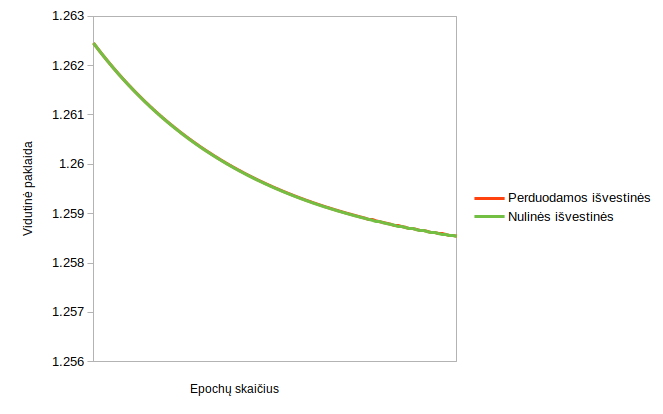
\includegraphics{images/paklaida.png}}
\caption{Apmokymo paklaidos.}
\label{fig:paklaidos1}
\end{figure}

Tinklą apmokant naudojant abu būdus, tinklo apmokymo klaidos funkcijų grafikai yra identiški, todėl nėra būtina šių paklaidų perduoti atliekant naują apmokymą.

\item \textbf{Lyginsiu tinklo vidutines paklaidas priklausant nuo apmokymų skačiaus su skirtingomis $\alpha$ ir $\eta$ reikšmėms.}


\item \textbf{Lyginsiu tinklo apmokymo vidutines paklaidas didėjant apmokymo duomenų kiekiui.}


\item \textbf{Atliksiu tinklo apmokymo greitaveikos tyrimą, esant skirtingoms tinklo topologijoms.}




\end{enumerate}
